\chapter{Progettazione Architetturale e di Dominio}

Il processo di transizione dall'analisi dei requisiti alla progettazione ha seguito i principi dell'Object-Oriented Design (OOD) e l'approccio BCE (Boundary-Control-Entity). In questo capitolo viene dettagliata la struttura statica del Domain Model, ponendo particolare enfasi sull'applicazione dei Design Pattern fondamentali per garantire la manutenibilità, l'estensibilità e il disaccoppiamento del sistema.

\section{Architettura a Strati e BCE}
L'architettura è organizzata in strati coerenti con il paradigma BCE. Le interazioni tra Boundary (CLI e mockup), Control (Controllers) ed Entity (Domain Model) sono strettamente direzionali, mentre la persistenza è isolata nel layer DAO.

\begin{figure}[H]
    \centering
    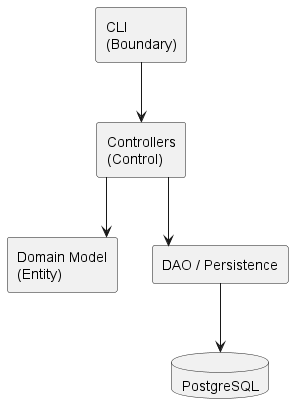
\includegraphics[width=\textwidth]{images/component_diagram.png}
    \caption{Architettura a strati e separazione BCE}
    \label{fig:component_diagram}
\end{figure}

\section{Package Diagram e Dipendenze}
Il Package Diagram (Figura \ref{fig:package_diagram}) descrive la struttura logica del progetto e le dipendenze tra i package principali. La CLI accede esclusivamente ai Controllers, i quali orchestrano Domain Model e DAO, mantenendo un flusso di dipendenze unidirezionale.

\begin{figure}[H]
    \centering
    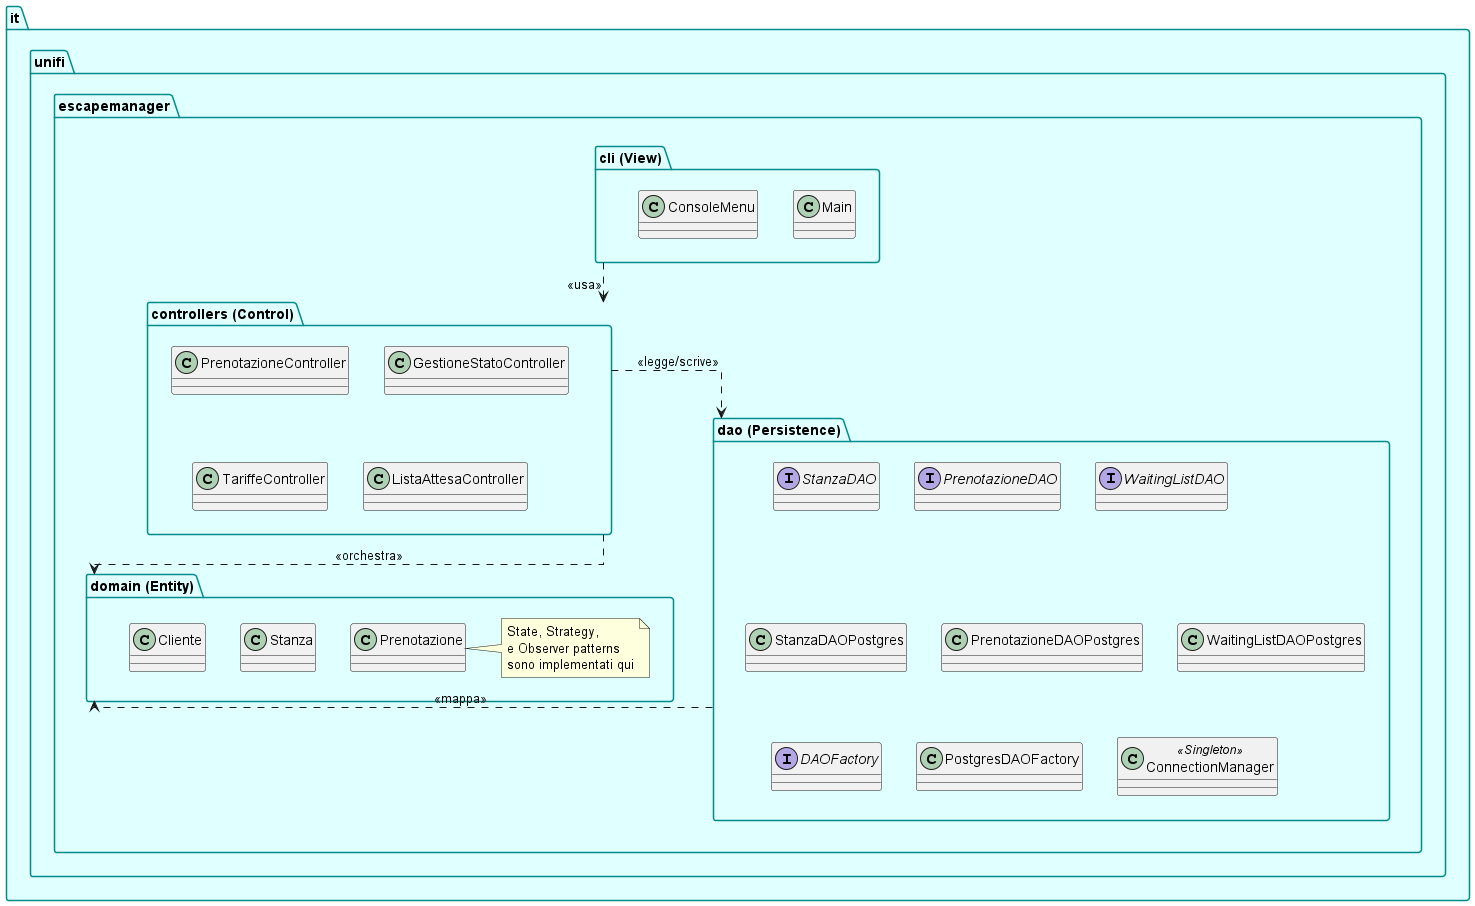
\includegraphics[width=0.75\textwidth]{images/package_diagram.png}
    \caption{Package Diagram dell'architettura di sistema}
    \label{fig:package_diagram}
\end{figure}

\section{Scelte Progettuali e Trade-off}
Ecco alcune scelte chiave adottate per mantenere il codice pulito e comprensibile:
\begin{itemize}
    \item \textbf{DAO + JDBC} invece di ORM: architettura leggera studiata per garantire maggiore controllo sul mapping e totale trasparenza dei flussi dati.
    \item \textbf{CLI come Boundary} per ridurre l'impatto della UI e concentrare lo sforzo sulla logica di business.
    \item \textbf{Pattern GoF espliciti} (State/Strategy/Observer) per rendere evidenti i punti di estensione del dominio.
    \item \textbf{Single Table Inheritance} per la gerarchia \texttt{Utente}, semplificando query e autenticazione futura.
\end{itemize}

\section{Domain Model (Class Diagram)}

La Figura \ref{fig:domain_model} illustra il diagramma delle classi per il nucleo dell'applicazione (Entity layer). Il modello non include volutamente i dettagli legati all'accesso ai dati (DAO) o all'interfaccia utente (View/CLI), concentrandosi esclusivamente sulle regole del franchise.

\begin{figure}[H]
    \centering
    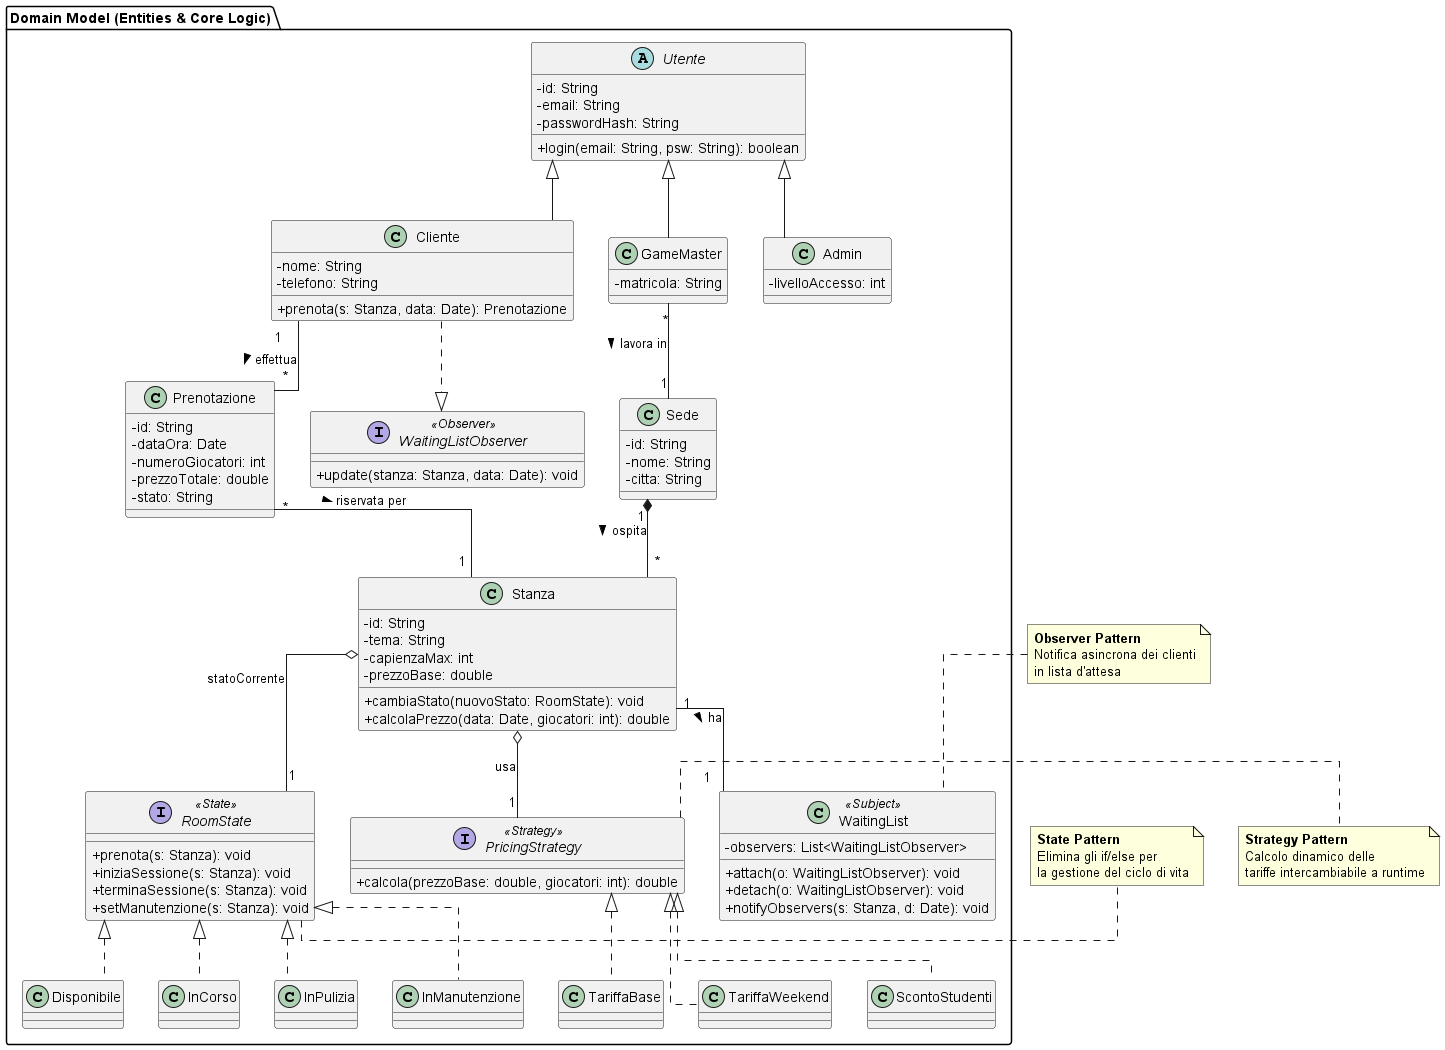
\includegraphics[width=1\textwidth]{images/domain_model.png}
    \caption{Diagramma delle Classi del Domain Model con Design Pattern}
    \label{fig:domain_model}
\end{figure}

\section{Class Diagram dei Controller e Boundary}
Per documentare i layer di controllo e presentazione, la Figura \ref{fig:class_diagram_controllers} mostra invece i Controllers (il livello Control) e la CLI (il livello Boundary).

\begin{figure}[H]
    \centering
    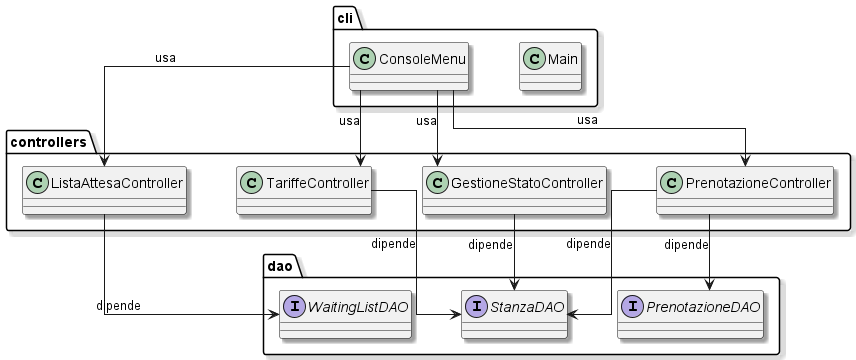
\includegraphics[width=0.9\textwidth]{images/class_diagram_controllers.png}
    \caption{Class Diagram: Controllers e Boundary (CLI)}
    \label{fig:class_diagram_controllers}
\end{figure}

\section{Class Diagram del Package DAO (Persistenza)}
Per non legare i Controller direttamente al database Postgres, il sistema usa il pattern \textbf{Abstract Factory} (DAO Factory). La Figura \ref{fig:class_diagram_dao} mostra il package \texttt{dao}, con le interfacce, le classi concrete e la connessione unica (Singleton).

\begin{figure}[H]
    \centering
    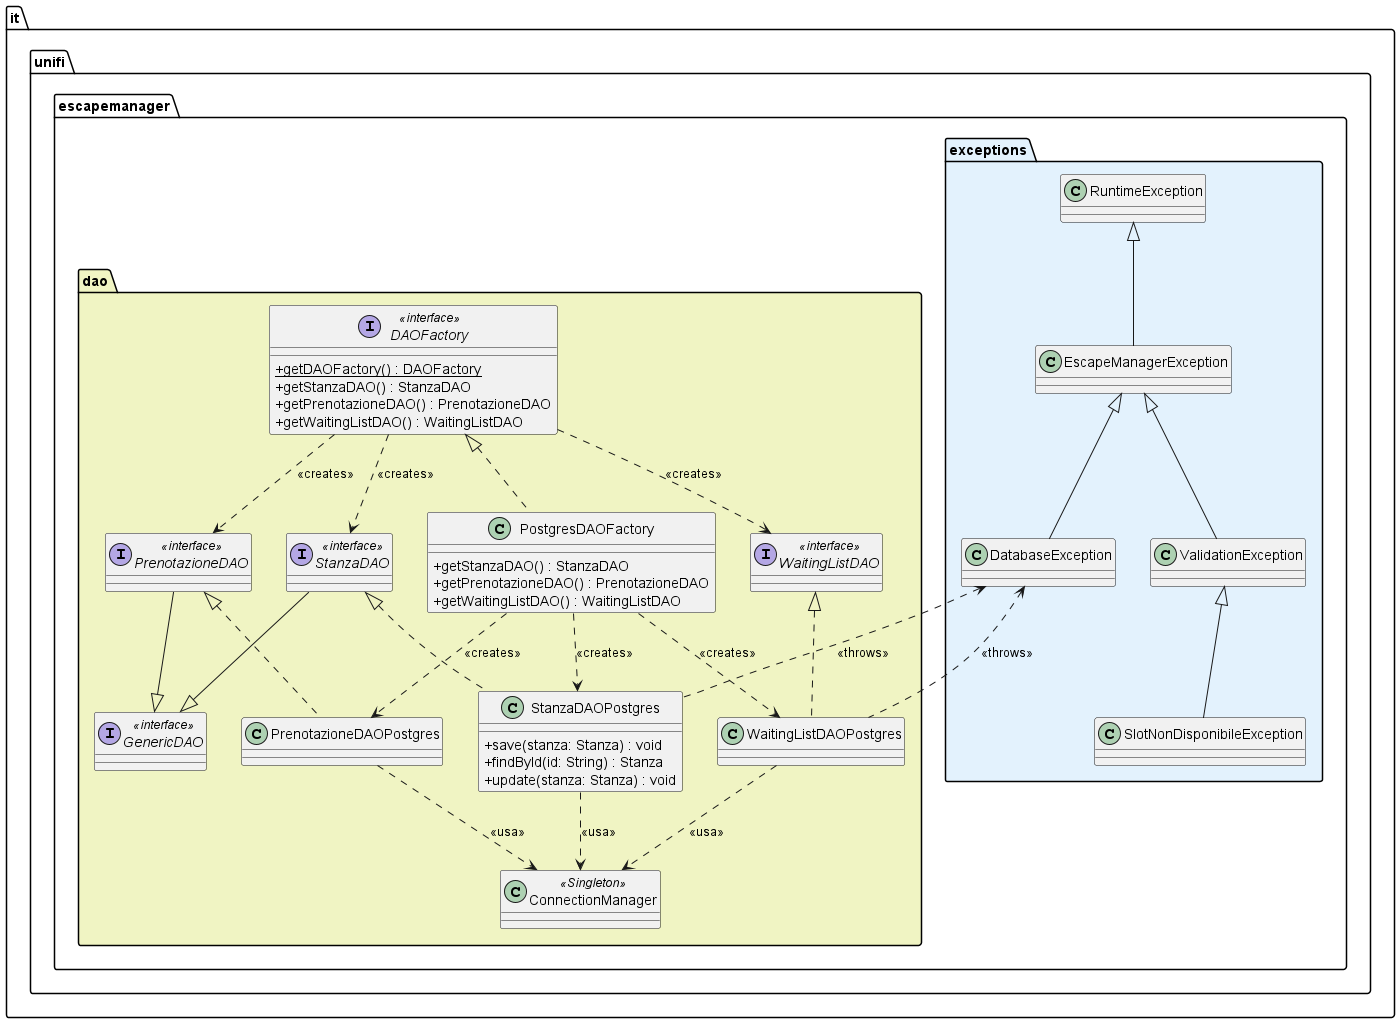
\includegraphics[width=0.95\textwidth]{images/class_diagram_persistence.png}
    \caption{Class Diagram: Package DAO e Gerarchia delle eccezioni}
    \label{fig:class_diagram_dao}
\end{figure}

\subsection{Scelte Architetturali e Design Pattern}

Per risolvere i problemi principali visti nei casi d'uso (Capitolo 2), ho inserito a livello di dominio tre Design Pattern della \textit{Gang of Four (GoF)}:

\begin{itemize}
    \item \textbf{State Pattern (Gestione ciclo di vita):} Come emerso nell'UC3, la \texttt{Stanza} attraversa fasi operative rigide (Disponibile, In Corso, In Pulizia, In Manutenzione). Invece di delegare il controllo a complessi blocchi \texttt{switch/case} basati su stringhe o enumerazioni, lo stato è stato reificato nell'interfaccia \texttt{RoomState}. Questo garantisce il rispetto del principio \textit{Open-Closed}: l'aggiunta di un nuovo stato futuro non richiederà la modifica del codice della classe \texttt{Stanza}.
    
    \item \textbf{Strategy Pattern (Politiche di Prezzo):} Le regole di tariffazione dipendono da fattori esterni (giorno della settimana, festività, tipologia di clienti). La classe \texttt{Stanza} delega il calcolo del costo totale all'interfaccia \texttt{PricingStrategy}. L'amministratore (UC4) può così iniettare a runtime strategie diverse (es. \texttt{TariffaBase} e \texttt{TariffaWeekend}) variando l'algoritmo di calcolo in modo trasparente.
    
    \item \textbf{Observer Pattern (Lista d'Attesa asincrona):} Per soddisfare il requisito dell'UC2 (Iscrizione Lista d'Attesa), è stato predisposto un meccanismo di Publish-Subscribe. La classe \texttt{WaitingList} agisce da \textit{Subject}, mantenendo una lista di \texttt{WaitingListObserver} (interfaccia implementata dal \texttt{Cliente}). L'infrastruttura di iscrizione è implementata e persiste su database; l'invio automatico delle notifiche è considerato un'estensione futura.
\end{itemize}

Oltre ai pattern, si sottolinea l'uso dell'ereditarietà per la gestione degli attori (\texttt{Utente} come classe astratta generalizzata) e la presenza di un riferimento a \texttt{Sede} tramite \texttt{sede\_id} nel modello dati, che consente di mantenere la coerenza con il concetto di franchising pur non essendo oggetto di operazioni dirette nella CLI.

\subsection{Object Diagram: Istanza Runtime del Pattern Observer}

Per illustrare concretamente il funzionamento del \textbf{Pattern Observer} (descritto nel Domain Model), la Figura \ref{fig:object_diagram} mostra un \textit{Object Diagram} rappresentativo di una specifica configurazione runtime del sistema.

\begin{figure}[H]
    \centering
    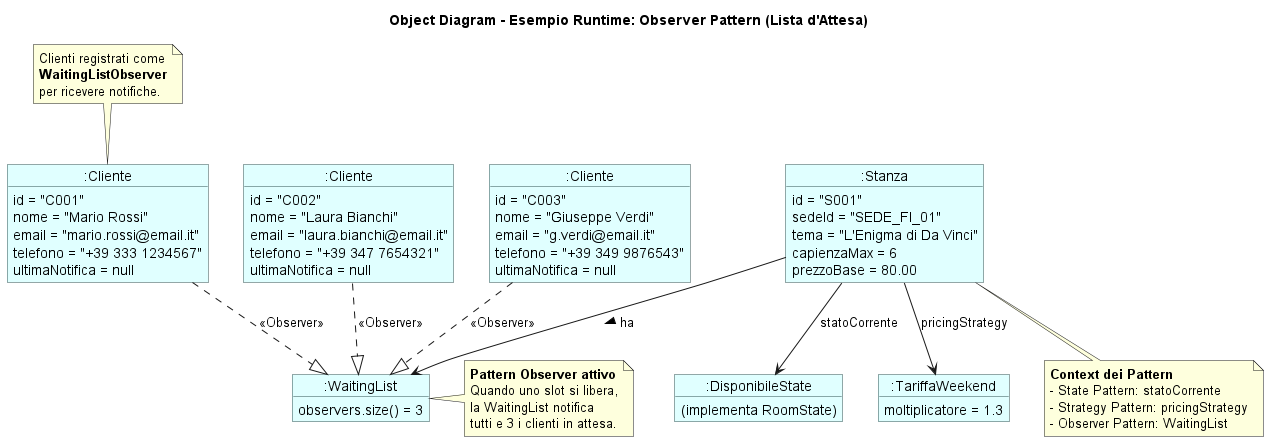
\includegraphics[width=0.95\textwidth]{images/object_diagram.png}
    \caption{Object Diagram: Esempio di istanza runtime del Pattern Observer (Lista d'Attesa)}
    \label{fig:object_diagram}
\end{figure}

L'Object Diagram raffigura tre clienti (\texttt{:Cliente}) registrati come osservatori (\texttt{WaitingList}\allowbreak\texttt{Observer}) sulla \texttt{:WaitingList} associata a una stanza specifica (\texttt{:Stanza}). Quando lo slot richiesto si libera, il Subject (\texttt{WaitingList}) invocherà il metodo \texttt{update()} su tutti e tre gli Observer, notificandoli della disponibilità.

Questo diagramma evidenzia inoltre le relazioni con i pattern \textbf{State} (stato corrente della stanza) e \textbf{Strategy} (politica di prezzo dinamica), mostrando come i tre pattern collaborino a runtime per realizzare la logica di business del franchising.

\subsection{State Machine Diagram}
Per documentare formalmente il ciclo di vita operativo della Stanza, è stato prodotto il diagramma a stati della Figura \ref{fig:state_machine_room}. Questo diagramma è una vista complementare al class diagram del Domain Model e descrive le transizioni valide tra i 4 stati concreti dell'interfaccia \texttt{RoomState}.

\begin{figure}[H]
    \centering
    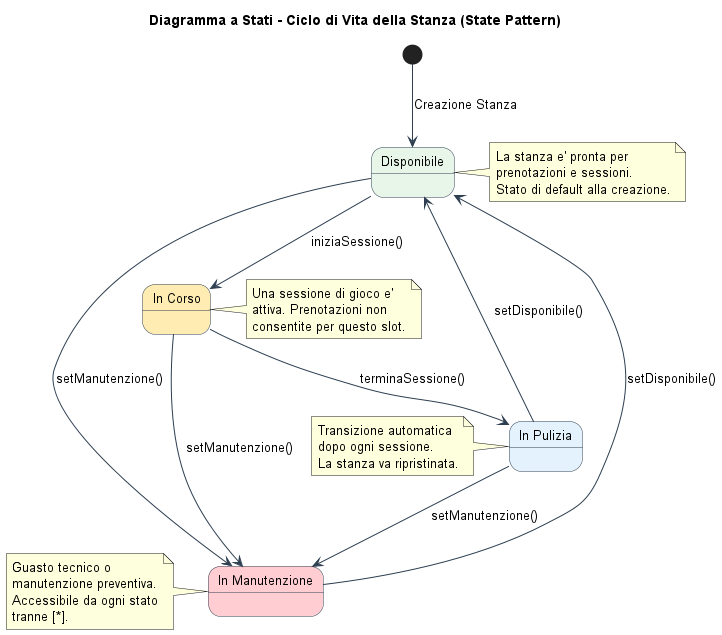
\includegraphics[width=0.85\textwidth]{images/state_machine_room.png}
    \caption{State Machine Diagram per il ciclo di vita della Stanza (RoomState)}
    \label{fig:state_machine_room}
\end{figure}


\section{Progettazione del Database}

Per salvare i dati, il Domain Model a oggetti è stato convertito in un database relazionale (PostgreSQL) usando specifiche strategie di mapping.

\subsection{Diagramma Entity-Relationship}

La Figura \ref{fig:er_diagram} mostra il diagramma Entità-Relazione (ER) del database, illustrando le tabelle principali, le chiavi primarie (PK) e i vincoli di chiave esterna (FK).

\begin{figure}[H]
    \centering
    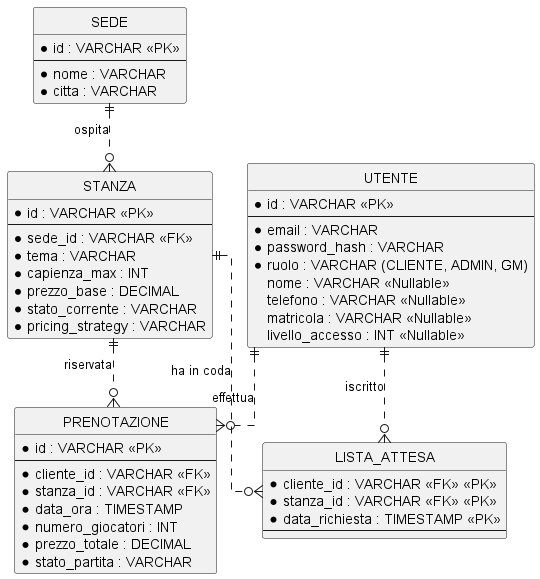
\includegraphics[width=0.85\textwidth]{images/er_diagram.png}
    \caption{Diagramma Entity-Relationship (ER) del sistema}
    \label{fig:er_diagram}
\end{figure}

\subsection{Strategie di Mapping e Modello Logico}

Per collegare il mondo a oggetti a quello delle tabelle ho scelto queste strade:

\begin{itemize}[leftmargin=*]
\raggedright
\setlength{\emergencystretch}{3em}
    \item \textbf{Mapping dell'Ereditarietà (Single Table Strategy):} La gerarchia della classe astratta \texttt{Utente} (Cliente, GameMaster, Admin) è stata mappata utilizzando il pattern \textit{Single Table Inheritance}. È stata creata un'unica tabella \texttt{UTENTE} provvista di una colonna discriminante (\texttt{ruolo}). Gli attributi specifici delle sottoclassi (es. \texttt{matricola} per il Game Master o \texttt{telefono} per il Cliente) sono stati resi \textit{nullable}. Questa scelta ottimizza le query di autenticazione evitando costose operazioni di \texttt{JOIN}.
    
    \item \textbf{Mapping dei Design Pattern (State e Strategy):} Le interfacce \texttt{RoomState} e \texttt{PricingStrategy} non diventano tabelle separate. Nella tabella \texttt{STANZA} sono persistite tramite stringhe (ad es.\ \texttt{stato\_corrente\allowbreak=\allowbreak IN\_MANUTENZIONE}). A livello di codice Java, i Data Access Object (DAO) utilizzano un meccanismo di \textit{Factory} per istanziare l'oggetto concreto corrispondente al valore letto dal database.
    
    \item \textbf{Associazioni Molti-a-Molti (Observer Pattern):} La logica Publish-Subscribe della Lista d'Attesa (UC2) si traduce relazionalmente nella tabella di \textit{junction} \texttt{LISTA\_ATTESA}. Questa tabella mappa la relazione N:N tra Clienti e Stanze, utilizzando una chiave primaria composita formata dalle foreign key e dal timestamp della richiesta.
\end{itemize}

\vspace{0.3cm}
\noindent Di seguito viene riportato lo \textbf{Schema Logico Relazionale} formalizzato:

\begin{itemize}[leftmargin=*]
\emergencystretch=3em
    \item \textbf{SEDE}(\underline{id}, nome, citta)
    \item \textbf{STANZA}(\underline{id}, \dashuline{sede\_id}, tema, capienza\_max, prezzo\_base, stato\_corrente, pricing\_strategy)
    \item \textbf{UTENTE}(\underline{id}, email, password\_hash, ruolo, nome*,\newline telefono*, matricola*, livello\_accesso*) --- {\small\textit{* attributo nullable a seconda del ruolo}}
    \item \textbf{PRENOTAZIONE}(\underline{id}, \dashuline{cliente\_id}, \dashuline{stanza\_id}, data\_ora, numero\_giocatori, prezzo\_totale, stato\_partita)
    \item \textbf{LISTA\_ATTESA}(\underline{\dashuline{cliente\_id}}, \underline{\dashuline{stanza\_id}}, \underline{data\_richiesta})
\end{itemize}

\section{Dinamica del Sistema (Implementation Perspective)}
Per illustrare le interazioni dinamiche tra gli oggetti a runtime, sono stati realizzati i Sequence Diagram per i casi d'uso principali.

\subsection{UC1 - Prenotazione Stanza}
La Figura \ref{fig:sequence_prenotazione} mostra il Sequence Diagram relativo al caso d'uso principale. Il diagramma evidenzia il rispetto del pattern architetturale BCE: l'interfaccia utente (Boundary) delega l'elaborazione al \texttt{PrenotazioneController} (Control), il quale orchestra il reperimento delle risorse persistenti e demanda la logica matematica di calcolo del prezzo all'entità \texttt{Stanza} (Entity). Particolare attenzione è stata posta nel disaccoppiamento del Controller dall'accesso ai dati, delegato interamente a un pattern creazionale.

\begin{figure}[H]
    \centering
    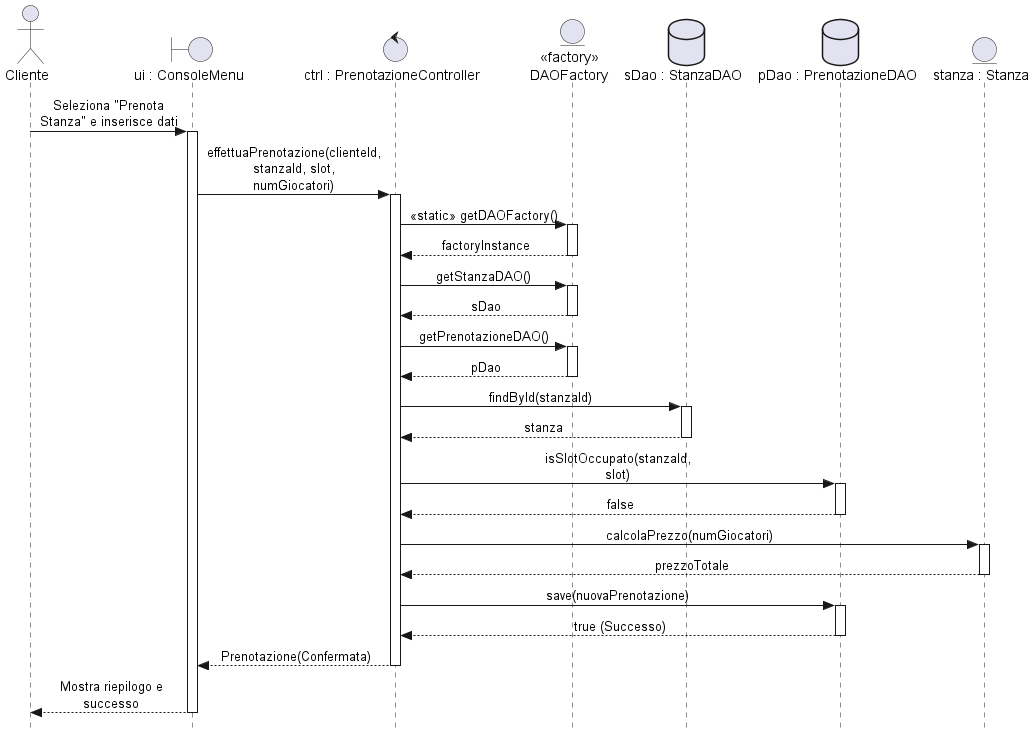
\includegraphics[width=\textwidth]{images/sequence_prenotazione.png}
    \caption{Sequence Diagram del caso d'uso UC1 (Prenotazione Stanza)}
    \label{fig:sequence_prenotazione}
\end{figure}

\subsection{UC4 - Configurazione Tariffe}
La Figura \ref{fig:sequence_tariffe} descrive il flusso di configurazione delle tariffe. L'Admin opera tramite la CLI, la quale delega al \texttt{TariffeController} la selezione della strategia e l'aggiornamento della stanza via DAO.

\begin{figure}[H]
    \centering
    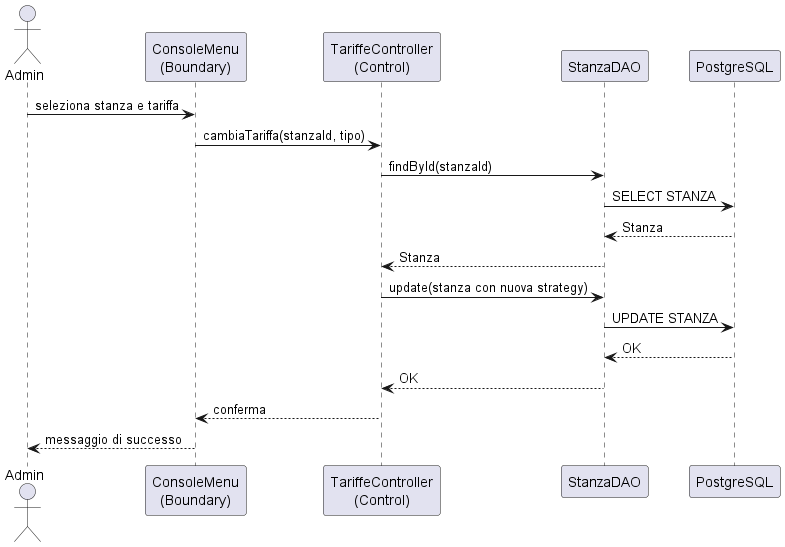
\includegraphics[width=0.95\textwidth]{images/sequence_tariffe.png}
    \caption{Sequence Diagram del caso d'uso UC4 (Configurazione Tariffe)}
    \label{fig:sequence_tariffe}
\end{figure}

\subsection{UC3 - Aggiornamento Stato Stanza}
La Figura \ref{fig:sequence_gestione_stato_cap3} mostra il Sequence Diagram per l'UC3, evidenziando la delega al \textbf{State Pattern}. Il Controller non contiene logica di stato: invoca il metodo di transizione sulla \texttt{Stanza}, la quale delega l'esecuzione all'oggetto \texttt{RoomState} corrente. Il diagramma include anche il flusso alternativo 4a (transizione non valida).

\begin{figure}[H]
    \centering
    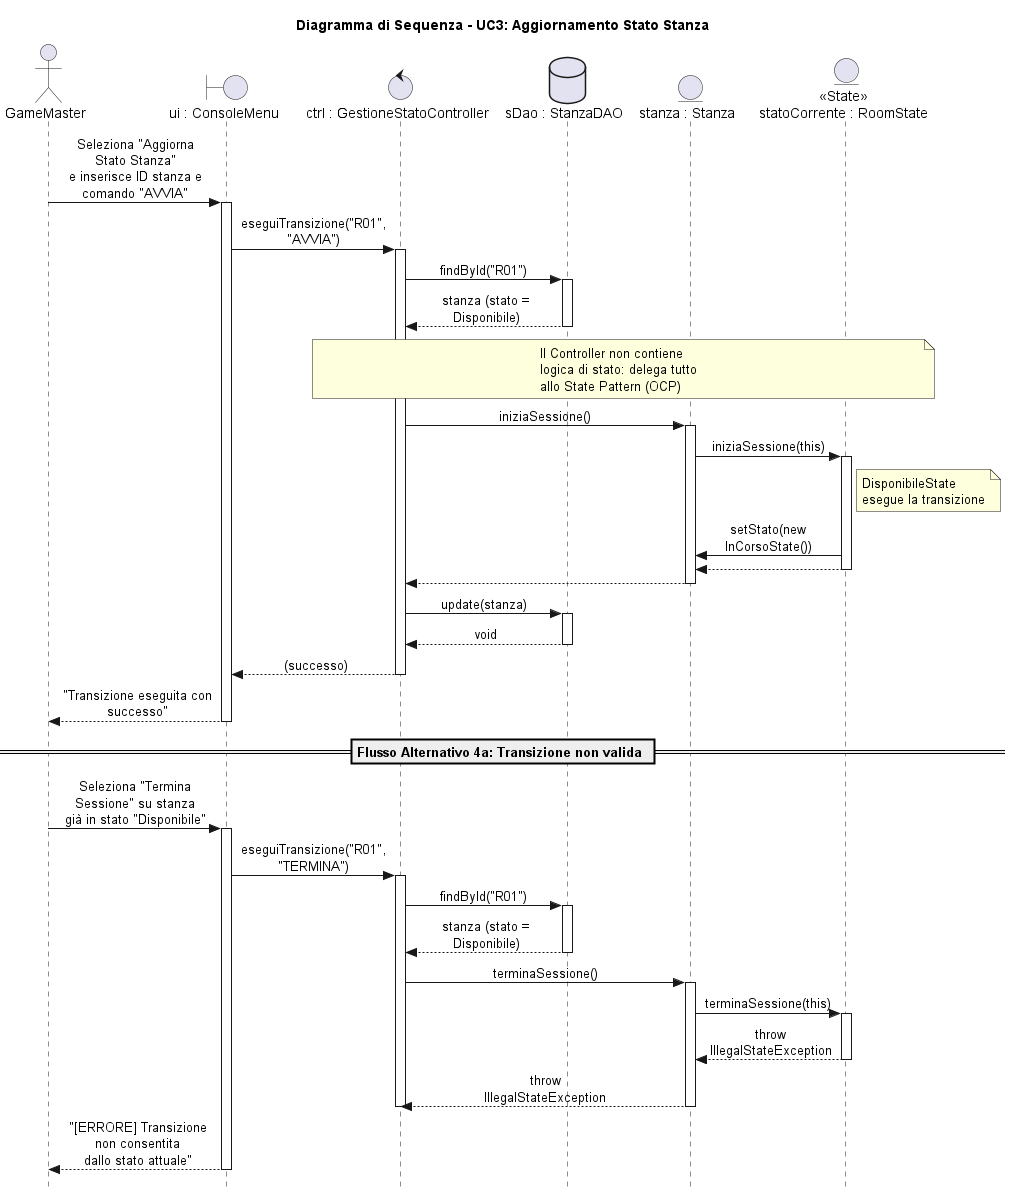
\includegraphics[width=0.95\textwidth]{images/sequence_gestione_stato.png}
    \caption{Sequence Diagram del caso d'uso UC3 (Aggiornamento Stato Stanza)}
    \label{fig:sequence_gestione_stato_cap3}
\end{figure}



\section{Pattern Creazionali: DAO Factory}
Nei diagrammi di sequenza si nota subito che, al momento di salvare i dati, ci si affida a una \textbf{DAO Factory} (Abstract Factory). 
L'idea è scollegare totalmente i Controller dal database PostgreSQL. Infatti, il Controller non crea mai una classe \texttt{StanzaDAOPostgres} usando \texttt{new}, ma si affida all'interfaccia esposta dalla Factory:

\begin{lstlisting}[language=Java, caption=Utilizzo del pattern DAO Factory nel Controller]
// Reperimento dinamico dei DAO indipendentemente dal DB sottostante
DAOFactory factory = DAOFactory.getDAOFactory();
StanzaDAO stanzaDao = factory.getStanzaDAO();
PrenotazioneDAO prenotazioneDao = factory.getPrenotazioneDAO();
\end{lstlisting}
Questo vuol dire che se un domani fosse necessario passare a MySQL, basterebbe creare una nuova Factory e i file SQL specifici, senza mai toccare il codice dei Controller o di Dominio.


